\documentclass[10pt,a4paper,twocolumns]{article}

\usepackage[utf8]{inputenc}
\usepackage{titling}
\usepackage{graphicx}
\usepackage{url}
\usepackage{appendix}
\usepackage[parfill]{parskip}
\usepackage{mathtools}
\usepackage[top=1cm,left=1cm,right=1cm,bottom=3cm]{geometry}
\usepackage{multicol}
\usepackage{caption}
\usepackage{fancyhdr}

\fancypagestyle{plain}{
	\fancyfoot[C]{
		\begin{minipage}{0.79\textwidth}
			\textbf{Acknowledgement}\\
			We would like to thank Nvidia for their donations to our lab.
		\end{minipage}
		\begin{minipage}{0.2\textwidth}
			
\includegraphics[width=1\textwidth]{logo_ntnu_eng}
		\end{minipage}
	}
}

\renewcommand{\headrulewidth}{0pt}
\pagenumbering{gobble}
\pagestyle{plain}

\newenvironment{Figure}
	{\par\medskip\noindent\minipage{\linewidth}}
	{\endminipage\par\medskip}
	
\begin{document}

	\begin{minipage}{0.2\textwidth}
		
\includegraphics[width=\textwidth]{hpc-lab-no-ntnu-logo}
	\end{minipage}
	\begin{minipage}{0.75\textwidth}
		\begin{center}
		{\huge Particle-In-Cell codes in CUDA}
		\end{center}
	\end{minipage}\\[0.5cm]

	\begin{center}
		Olav Emil Eiksund, Advisor: Dr. Anne C. Elster \\
		Department of Computer and Information Science
	\end{center}

	\begin{multicols*}{2}
		\section*{Introduction}
		 The objective of this project is to implement a PIC simulation
		 running on a GPU. The project is a continuation of earlier work
		 by Elster, Meyer and Larsgård. These have utilized MPI and
		 OpenMP for parallelization, and later on this project might
		 be used to provide a performance measure for CUDA.
		 
		\section*{PIC}
		\begin{multicols*}{2}
			The Particle-In-Cell method models the behaviour of charged
			particles in a grid, for example electrons or plasma.
			
			\begin{Figure}
				\center
				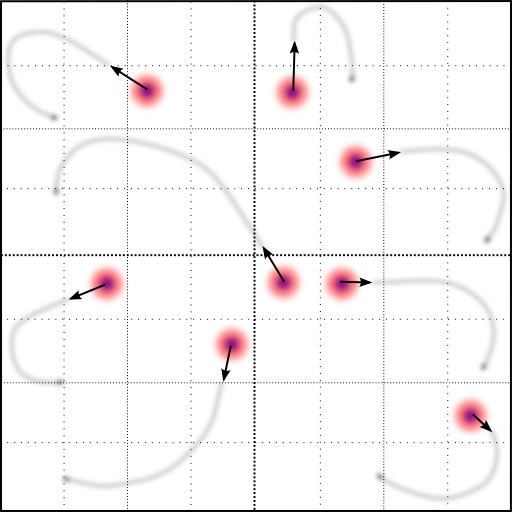
\includegraphics[width=0.8\textwidth]{pic_illustration.png}
				\captionof{figure}{Particles moving in cells}
				\label{fig:illustration}
			\end{Figure}
		\end{multicols*}
		
		\subsection*{Physics}
		The simulation is based on Poissons equation $\nabla^2\Phi=-\rho/\epsilon_0$,
		and lets us find the electric potential $\Phi$ from charge density $\rho$.
		We can in turn determine the electric field using $E=-\nabla\Phi$. Finally
		each particle's motion can be calculated from the electrical
		force acted upon it using laws of motion and electrical force.
		
		\subsection*{Algorithm}
		The steps of the simulation are:
		\begin{enumerate}
		\item	Find charge density. The charge of each particle is
		distributed among it's neighbour vertices.
		\item	Solve the field for potential. Poisson's equation is solved
		to find the electric potential.
		\item	Determine the electrical field. Computed using first order
		differences, the electrical field at each point is interpolated
		using the scheme below.
		\item	Move particles. With $a=F/m=E/(q\cdot m)$ we can
		update the velocity	and position of each particle. In this
		 implementation a leap-frog method is used.
		\end{enumerate}
		
		As the particles' positions are continous, and the calculations
		are performed on the discrete grid, charge contribution and
		electrical field strength has to be interpolated. Each
		neighbouring corner is weighted according to the particle's
		distance. For instance, charge contributed to $(i,j,k)$ is
		proportional to $(h_x-a)\cdot (h_y-b)\cdot (h_z-c)$, see figure below.
		
		\begin{Figure}
			\center
			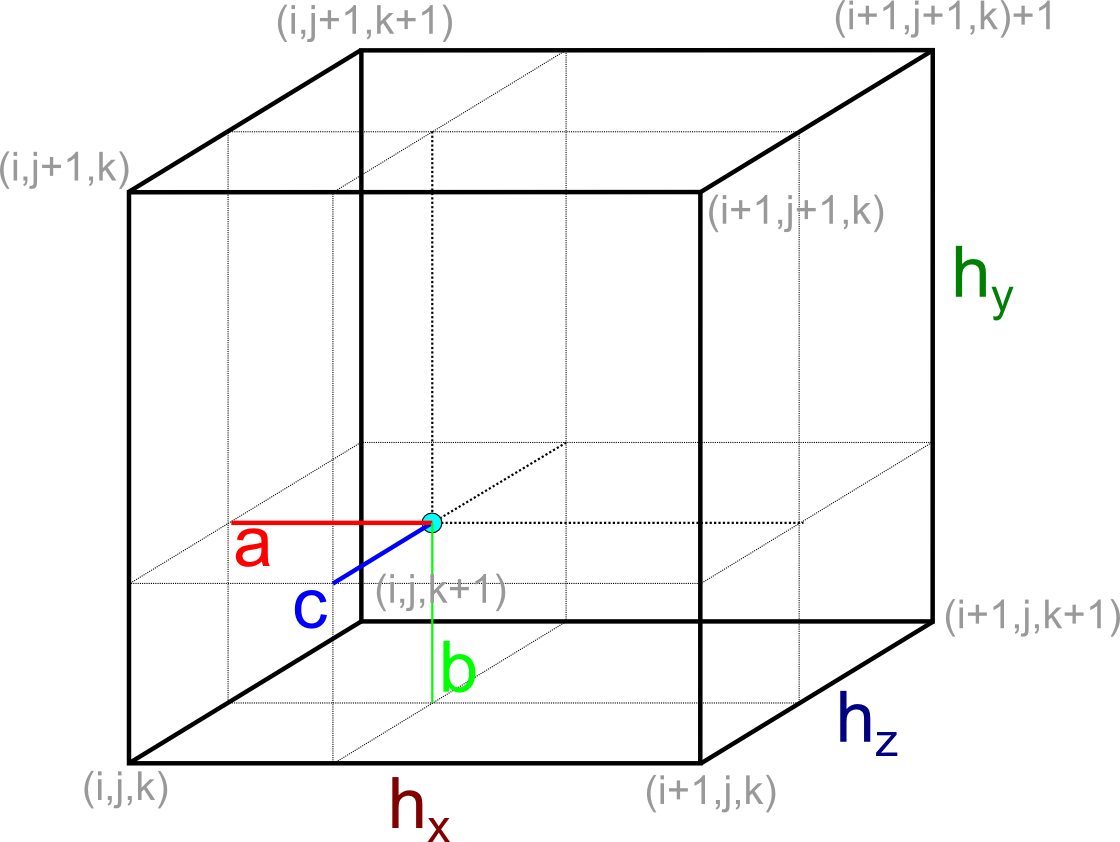
\includegraphics[width=0.8\textwidth]{grid.png}
			\captionof{figure}{Interpolating coordinates}
			\label{fig:interpolation}
		\end{Figure}
		
		\subsection*{Applications}
		Given sufficiently high resolution in the grid and small
		enough time steps, the simulation should correctly model
		phenomena such as plasma.
		
		While simulating the particles is an intuitive use of PIC
		other applications for solving Poissons equation exists, and
		with minor adjustments this solution could be adapted for
		other uses.
		
		\section*{Implementation}
		The implementation is relatively straightforward, with each
		step of the algorithm translating to a kernel call. The
		compute-intensive part of the simulation is the solver.
		Two different solvers are being implemented, a direct solver
		using cuFFT, and an iterative solver using SOR.
		
		\subsection*{cuFFT}
		CUDA's FFT library provides an efficient and easy to learn
		interface. With support for 1D, 2D and 3D transformations,
		this lets us implement a performant solver for PDE's.
		
	\end{multicols*}

\end{document}
